\section{Experiments}
\label{sec:experiments}

We present experiments on \MNIST \citep{LecunIEEE1998} and \Cifar \citep{Krizhevsky2009}. We first analyze the impact of fixed-point quantization schemes on robustness (\secref{subsec:experiments-quantization}). Subsequently, we discuss weight clipping (\Clipping, \secref{subsec:experiments-clipping}), showing that improved robustness originates from increased redundancy in the weight distribution. Then, we focus on random bit error training (\Random, \secref{subsec:experiments-randbet}). We show that related work \cite{KimDATE2018,KoppulaMICRO2019} does not generalize, while \Random generalizes across chips and voltages, as demonstrated on profiled bit error patterns from different chips. \secref{subsec:experiments-discussion} summarizes our results for various precisions $m$.

\begin{table}
	\centering
	\small 
	\caption{\textbf{Robust Quantization}. \RTE for random bit errors at $p = 0.05\%$ and $p = 0.5\%$
	for different quantization schemes, \cf \secref{subsec:robustness-quantization}. Minor differences
	can have large impact on \RTE while clean test error is unaffected. For $8$ bit the second row shows \Normal quantization (symmetric/per-layer) whereas the last row is our \Quant.
	*\Clipping[$0.1$]+\Quant with and without rounding.
	}
	\label{tab:quantization-robustness}
	\vspace*{-0.25cm}
	\hspace*{-0.2cm}
	\begin{tabular}{| c | l | c | c | c |}
		\hline
		\multicolumn{2}{|c|}{Quantization Schemes} & \multirow{2}{*}{\begin{tabular}{@{}c@{}}\TE\\in \%\end{tabular}}& \multicolumn{2}{c|}{\RTE in \%}\\
		\cline{4-5} 
		\multicolumn{2}{|c|}{(%\Normal on 
		\CifarT)} && $p{=}0.05$ & $p{=}0.5$\\
		\hline
		\hline
		\multirow{5}{*}{\rotatebox{90}{$8$ bit}} & \eqnref{eq:quantization}, global & 4.63 & 86.01 {\color{gray}\scriptsize ${\pm}$3.65} & 90.71 {\color{gray}\scriptsize ${\pm}$0.49}\\
		& \eqnref{eq:quantization}, per-layer & 4.36 & 5.51 {\color{gray}\scriptsize ${\pm}$0.19} & 24.76 {\color{gray}\scriptsize ${\pm}$4.71}\\
		& +asymmetric & 4.36 & 6.47 {\color{gray}\scriptsize ${\pm}$0.22} & {\color{colorbrewer1}40.78} {\color{gray}\scriptsize ${\pm}$7.56}\\
		& +unsigned & 4.42 & 6.97 {\color{gray}\scriptsize ${\pm}$0.28} & 17.00 {\color{gray}\scriptsize ${\pm}$2.77}\\
		& +rounding (=\Quant) & 4.32 & \bfseries 5.10 {\color{gray}\scriptsize ${\pm}$0.13} & \bfseries 11.28 {\color{gray}\scriptsize ${\pm}$1.47}\\
		\hline
		\hline
		\multirow{2}{*}{\rotatebox{90}{$4$ bit}} & w/o rounding* & 5.81 & 90.40 {\color{gray}\tiny ${\pm}$0.21} & 90.36 {\color{gray}\tiny ${\pm}$0.2}\\
		& w/ rounding* & \bfseries 5.29 & \bfseries 5.75 {\color{gray}\tiny ${\pm}$0.06} & \bfseries 7.71 {\color{gray}\tiny ${\pm}$0.36}\\
		\hline
	\end{tabular}
	\vspace*{-0.2cm}
\end{table}

\textbf{Metrics:} We report (clean) test error \TE (lower is better, $\downarrow$), corresponding to \emph{clean} weights, and \textbf{robust test error \RTE} ($\downarrow$) which is the 
\textbf{test error after injecting bit errors into the weights}. As the
bit errors are random we report the \emph{average} \RTE and its standard deviation for $50$ samples of random bit errors with rate $p$ as detailed in \secref{sec:errors}.

\textbf{Architecture:} We use SimpleNet \citep{HasanpourARXIV2016}, providing comparable performance to ResNets \cite{HeCVPR2016} with only $W{=}5.5\text{Mio}$ weights on \CifarT. On \MNIST, we halve all channel widths, resulting in roughly $1\text{Mio}$ weights. On \CifarH, we use a Wide ResNet (WRN) \cite{ZagoruykoBMVC2016}. As batch normalization (BN) \cite{IoffeICML2015} yields
consistently worse robustness against bit errors we use group normalization (GN) \cite{WuECCV2018}, see 
\appref{subsec:supp-experiments-bn}.

\textbf{Training:} We use stochastic gradient descent with an initial learning rate of $0.05$, multiplied by $0.1$ after $\nicefrac{2}{5}$, $\nicefrac{3}{5}$ and $\nicefrac{4}{5}$ of $100$/$250$ epochs on \MNIST/\Cifar. On \Cifar, we whiten the input images and use AutoAugment \cite{CubukARXIV2018} with Cutout \cite{DevriesARXIV2017}. For \Random, random bit error injection starts when the loss is below 1.75 on \MNIST/\CifarT or 3.5 on \CifarH. Normal training with the standard and our robust quantization are denoted \Normal and \Quant, respectively. Weight clipping with $\wmax$ is referred to as \Clipping[\wmax] or together with \Random as \Random[\wmax]. 
For \Quant, $m = 8$, we obtain $4.3\%$ on \CifarT and $18.5\%$ \TE on \CifarH. On \MNIST, $0.47\%$ are possible even for $m = 2$. 

\begin{table}
	\centering
	\caption{\textbf{Weight Clipping Robustness.} Clean \TE and \RTE as well as clean confidence and confidence at $p{=}1\%$ bit errors (in \%, higher is better, $\uparrow$) for \Clipping and \Clipping with label smoothing (+LS). \TE increases for $\wmax = 0.025$ where the DNN is not able to produce large (clean) confidences. LS consistently reduces robustness, indicating that robustness is due to enforcing high confidence during training \emph{and} weight clipping.}
	\label{tab:clipping-robustness}
	\vspace*{-0.25cm} 
	\small 
	\hspace*{-0.2cm}
	\begin{tabular}{| l | c | c | c | c | c |}
		\hline
		Model & \multirow{2}{*}{\begin{tabular}{@{}c@{}}\TE\\in \%\end{tabular}} & \multirow{2}{*}{\begin{tabular}{@{}c@{}}Conf\\in \%\end{tabular}} & \multirow{2}{*}{\begin{tabular}{@{}c@{}}Conf\\$p{=}1$\end{tabular}} & \multicolumn{2}{c|}{\RTE in \%}\\
		\cline{5-6}
		(\CifarT) & & & & $p{=}0.1$ & $p{=}1$\\
		\hline 
		\hline
		\Quant & \bfseries 4.32 & \bfseries 97.42 & 78.43 & 5.54 & 32.05\\
		\hline
		\Clipping[$0.15$] & 4.42 & 96.90 & 88.41 & \bfseries  5.31 & 13.08\\
		\Clipping[$0.1$] & 4.82 & 96.66 & 92.97 & 5.58 & 8.93\\
		\Clipping[$0.05$] & 5.44 & 95.90 & \bfseries 94.73 & 5.90 & \bfseries 7.18\\
		\Clipping[$0.025$] & 7.10 & {\color{colorbrewer1}84.69} & 83.28 & 7.40 & 8.18\\
		\hline
		\Clipping[$0.15$]+LS & 4.67 & 88.22 & 47.55 & 5.83 & {\color{colorbrewer2}29.40}\\
		\Clipping[$0.1$]+LS & 4.82 & 87.90 & 78.89 & 6.10 & 10.59\\
		\Clipping[$0.05$]+LS & 5.30 & 87.41 & 85.04 & 6.43 & 7.30\\
		\hline
	\end{tabular}
	\vspace*{-0.2cm}
\end{table}

Our \textbf{appendix} includes implementation details (\appref{sec:supp-implementation}), more information on our experimental setup (\appref{subsec:supp-experiments-setup}), and complementary experiments (\appref{sec:supp-experiments}). Among others, we discuss the robustness of BN (\appref{subsec:supp-experiments-bn}), other architectures such as ResNet-50 (\appref{subsec:supp-experiments-bn}), qualitative results for \Clipping (\appref{subsec:supp-experiments-clipping}) and complete results for $m = 4,3,2$ bits precision (\appref{subsec:supp-experiments-summary}). Also, we discuss a simple guarantee how the average \RTE relates
to the true expected robust error (\appref{subsec:supp-bound}). Our \textbf{code} will be made publicly available.

\subsection{Quantization Choice Impacts Robustness}
\label{subsec:experiments-quantization}

Quantization schemes affect robustness significantly, even when not affecting accuracy. 
\tabref{tab:quantization-robustness} shows that per-layer quantization reduces \RTE significantly for small bit error rates, \eg, $p = 0.05\%$. While asymmetric quantization further reduces the quantization range, \RTE increases, especially for large bit error rates, \eg, $p = 0.5\%$ (marked in {\color{colorbrewer1}red}). This is despite \figref{fig:quantization} showing a slightly smaller impact of bit errors. This is caused by an asymmetric quantization into \emph{signed} integers: Bit flips in the most significant bit (MSB, \ie, sign bit) are not meaningful if the quantized range is not symmetric as the sign bit does not reflect the sign of the represented weight value, see \appref{subsec:supp-experiments-quantization}. Similarly, replacing integer conversion of $\nicefrac{w_i}{\Delta}$ by proper rounding, $\lceil\nicefrac{w_i}{\Delta}\rfloor$, reduces \RTE significantly (resulting in our \Quant).
This becomes particularly important for $m = 4$. Here, rounding also improves clean \TE slightly, but the effect is significantly less pronounced. Proper rounding generally reduces the quantization error. However, it is striking that this has little impact on \TE but tremendous effect on \RTE.
For $m = 4$ or lower, we also found weight clipping to help training, obtaining lower \TE.
Overall, random bit errors induce unique error distributions, \cf \figref{fig:quantization}, heavily dependent on quantization details.

\begin{table}[t]
	\centering
	\caption{\textbf{Fixed Pattern Bit Error Training.} \RTE for training on an entirely fixed bit error pattern (\Pattern). \emph{Top:} Evaluation on the same pattern; \Pattern trained on $p = 2.5\%$ does not generalize to $p = 1\%$ even though the bit errors for $p = 1\%$ are a subset of those seen during training for $p = 2.5\%$ (in {\color{colorbrewer1}red}). \emph{Bottom:} \Pattern also fails to generalize to completely random bit errors. This can be confirmed on profiled bit errors in \appref{subsec:supp-randbet-baselines}.}
	\label{tab:randbet-baselines}
	\vspace*{-0.25cm}
	\small
	\begin{tabular}{| l | c | c |}
		\hline
		Model (\CifarT) & \multicolumn{2}{c|}{\RTE in \%, $p$ in \%}\\
		\hline
		\hline
		\textbf{Evaluation on Fixed Pattern} & $p{=}1$ & $p{=}2.5$\\
		\hline
		\Pattern $p{=}2.5$ & {\color{colorbrewer1}14.14} & 7.87\\
		\Pattern[$0.15$] $p{=}2.5$ & {\color{colorbrewer1}8.50} & 7.41\\
		\hline\hline
		\textbf{Evaluation on \emph{Random} Patterns} & $p{=}1$ & $p{=}2.5$\\
		\hline
		\Pattern[$0.15$] $p{=}2.5$ & 12.09 & 61.59\\
		\hline
	\end{tabular}
	\vspace*{-0.2cm}
\end{table}

\subsection{Weight Clipping Improves Robustness}
\label{subsec:experiments-clipping}
While the quantization range adapts to the weight range
after every update during training, weight clipping explicitly constraints the weights to $[-\wmax, \wmax]$.
\tabref{tab:clipping-robustness} shows the effect of
different $\wmax$ for \CifarT with 8 bit precision. The clean test error is not affected for \Clipping[$\mathbf{\wmax{=}0.15}$] but
one has already strong robustness improvements for $p=1\%$
compared to \Quant (\RTE of 13.18\% vs 32.05\%). Further reducing $\wmax$ leads to a slow increase in clean \TE and decrease in average clean confidence, while significantly
improving \RTE to $7.18\%$ for $p=1\%$ at $\wmax=0.05$. For $\wmax=0.025$
the DNN is no longer able to achieve high confidence (marked in {\color{colorbrewer1}red}) which leads to stronger loss of clean \TE. Interestingly, the gap between clean and perturbed confidences under bit errors for $p=1\%$ is (almost) monotonically decreasing. These findings generalize to other datasets and precisions, see \appref{subsec:supp-experiments-summary}. However, for low precision $m\leq 4$ the effects are stronger 
as \Quant alone does not yield any robust models and weight clipping is essential for achieving robustness. 

As discussed in \secref{subsec:robustness-clipping} the robustness of the DNN originates in the cross-entropy loss enforcing high confidences on the training set and, thus, large logits while weight clipping works against having large logits. Therefore, the network has to utilize more weights with larger absolute values (compared to $\wmax$).
In order to test this hypothesis, we limit the confidences that need to be achieved via label smoothing \cite{SzegedyCVPR2016}, targeting $0.9$ for the true class and $\nicefrac{0.1}{9}$ for the other classes. According to \secref{subsec:robustness-clipping}, this should lead to less robustness, as the DNN has to use ``fewer'' weights. Indeed, in \tabref{tab:clipping-robustness}, \RTE at $p=1\%$ increases from $13.08\%$ for \Clipping[$0.15$] to $29.4\%$ when using label smoothing (marked in {\color{colorbrewer2}blue}). Moreover, the difference between average clean and perturbed confidence is significantly larger for DNNs trained with label smoothing. 

In \appref{subsec:supp-experiments-clipping} we show that robustness against bit errors also leads to robustness against $L_\infty$ perturbations which generally affect all weights in contrast to random bit errors, and provide more qualitative results about the change of the weight distribution induced by clipping in \figref{fig:supp-clipping}.

\begin{table}[t]
	\centering
	\small
	\caption{\textbf{Random Bit Error Training (\Random).} Average \RTE (and standard deviation) of \Random evaluated at various bit error rates $p$ and using $m = 8$ or $4$ bit precision. For low $p$, weight clipping provides sufficient robustness. However for $p \geq 0.5$, \Random increases robustness significantly. This is pronounced for lower precisions.}
	\label{tab:randbet-robustness}
	\vspace*{-0.25cm}
	\hspace*{-0.25cm}
	\begin{tabular}{|@{\hskip 3px}c@{\hskip 3px}|@{\hskip 3px}l@{\hskip 3px}|@{\hskip 3px}c@{\hskip 3px}|@{\hskip 3px}c@{\hskip 3px}|@{\hskip 3px}c@{\hskip 3px}|@{\hskip 3px}c@{\hskip 3px}|}
		\hline
		& Model (\CifarT) & \multirow{2}{*}{\begin{tabular}{@{}c@{}}\TE\\in \%\end{tabular}} &\multicolumn{3}{c|}{\RTE in \%}\\
		\cline{4-6}
		& $\mathbf{\wmax{=}0.1}$, $p$ in \% && $p{=}0.5$ & $p{=}1$ & $p{=}1.5$\\
		\hline
		\hline
		\multirow{5}{*}{\rotatebox{90}{$8$bit}} & \Quant & \bfseries 4.32 & 11.28 {\color{gray}\tiny ${\pm}$1.47} & 32.05 {\color{gray}\tiny ${\pm}$6} & 68.65 {\color{gray}\tiny ${\pm}$9.23}\\
		& \Clipping & 4.82 & 6.95 {\color{gray}\tiny ${\pm}$0.24} & 8.93 {\color{gray}\tiny ${\pm}$0.46} & 12.22 {\color{gray}\tiny ${\pm}$1.29}\\
		& \Random $p{=}1$ & 4.90 & \bfseries 6.36 {\color{gray}\tiny ${\pm}$0.17} & \bfseries 7.41 {\color{gray}\tiny ${\pm}$0.29} & \bfseries 8.65 {\color{gray}\tiny ${\pm}$0.37}\\
		\hline
		\multirow{2}{*}{\rotatebox{90}{$4$bit}} & \Clipping & \bfseries 5.29 & 7.71 {\color{gray}\tiny ${\pm}$0.36} & 10.62 {\color{gray}\tiny ${\pm}$1.08} & 15.79 {\color{gray}\tiny ${\pm}$2.54}\\
		& \Random $p{=}1$ & 5.39 & \bfseries 7.04 {\color{gray}\tiny ${\pm}$0.21} & \bfseries 8.34 {\color{gray}\tiny ${\pm}$0.42} & \bfseries 9.77 {\color{gray}\tiny ${\pm}$0.81}\\
		\hline
	\end{tabular}
	\vspace*{-0.2cm}
\end{table}

\subsection{\Random Yields Generalizable Robustness}
\label{subsec:experiments-randbet}

\textbf{Training on Profiled Errors Does Not Generalize:}
%\label{subsec:experiments-baselines}
%
Co-design approaches such as \cite{KimDATE2018,KoppulaMICRO2019} combine training DNNs on profiled SRAM or DRAM bit errors with hardware-approaches to limit the errors' impact.
However, profiling SRAM or DRAM requires expensive infrastructure, expert knowledge and time. 
More importantly, training on profiled bit errors does not generalize to previously unseen bit error distributions (\eg, other chips or voltages): \tabref{tab:randbet-baselines} (top) shows \RTE of \Pattern, \ie, pattern-specific bit error training. The main problem is that \Pattern does \emph{not} even generalize to lower bit error rates (\ie, higher voltages) of the same pattern as trained on (marked in {\color{colorbrewer1}red}). This is striking as, following \figref{fig:errors}, the bit errors form a subset of the bit errors seen during training: training with $p = 2.5\%$ bit errors does not provide robustness for $p = 1\%$, \RTE increases $7.9\%$ to $14.1\%$. It is not surprising, that \tabref{tab:randbet-baselines} (bottom) also demonstrates that \Pattern does not generalize to random bit error patterns: \RTE increases from $7.4\%$ to $61.6\%$ at $p = 2.5\%$. The same observations can be made when training on real, profiled bit errors corresponding to the chips in \figref{fig:errors}, see \appref{subsec:supp-randbet-baselines}.
Overall, obtaining robustness that generalizes across voltages \emph{and} chips is crucial for low-voltage operation to become practical.

\begin{table}[t]
	\centering
	\small
	\caption{\textbf{Generalization to Profiled Bit Errors.} \RTE for \Random on two different profiled chips. The bit error rates differ across chips due to measurements at different voltages, also see \figref{fig:errors}. Chip 2 exhibits a bit error distribution significantly different from uniform random bit errors: bit errors are strongly aligned along columns and biased towards $0$-to-$1$ flips, \cf \figref{fig:errors}. Nevertheless, \Random generalizes surprisingly well.}
	\label{tab:randbet-generalization}
	\vspace*{-0.25cm}
	\hspace*{-0.15cm}
	\begin{tabular}{| l | l | c | c |}
		\hline
		Chip (\figref{fig:errors}) & Model (\CifarT)& \multicolumn{2}{c|}{\RTE in \%}\\
		\hline
		\hline
		\bfseries Chip 1 && $p{\approx}0.86$ & {\color{colorbrewer1}$p{\approx}2.75$}\\
		\hline
		& \Random[$0.05$] $p{=}1.5$ & 7.04 & 9.37\\
		\hline
		\hline
		\bfseries Chip 2 && $p{\approx}0.14$ & {\color{colorbrewer1}$p{\approx}1.08$}\\
		\hline
		& \Random[$0.05$] $p{=}1.5$ & 6.00 & 9.00\\
		\hline
	\end{tabular}
	\vspace*{-0.2cm}
\end{table}
\begin{figure*}[t]
	\centering
	\vspace*{-0.1cm}
	\hspace*{-0.3cm}
	\begin{subfigure}{0.32\textwidth}
		\centering
		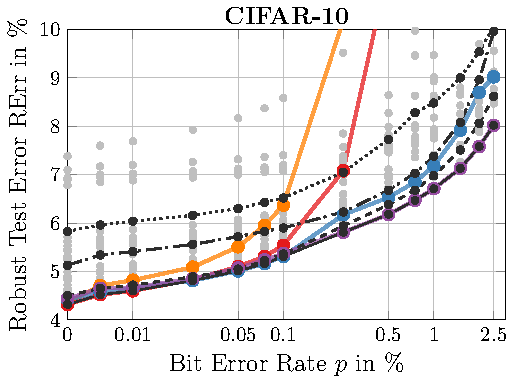
\includegraphics[width=5.75cm]{c10_pareto_8bit}
	\end{subfigure}
	\hfill
	\begin{subfigure}{0.32\textwidth}
		\centering
		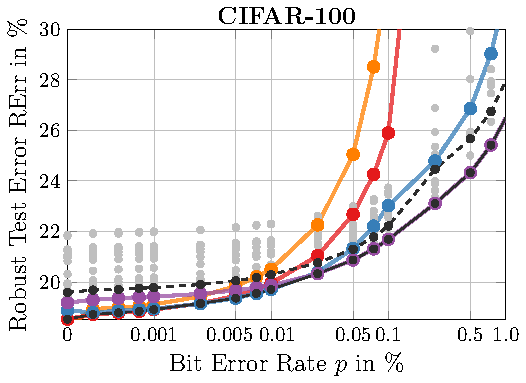
\includegraphics[width=5.75cm]{c100_pareto_8bit}
	\end{subfigure}
	\hfill
	\begin{subfigure}{0.32\textwidth}
		\centering
		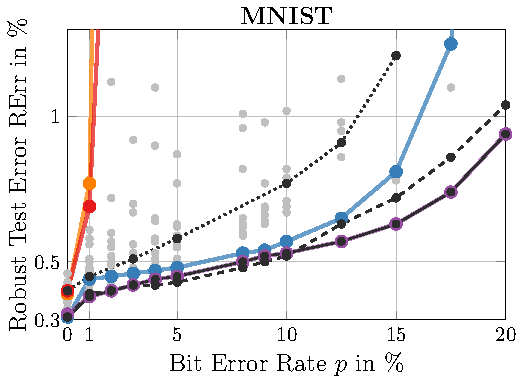
\includegraphics[width=5.75cm]{m_pareto_8bit}
	\end{subfigure}
	
	\hspace*{-0.1cm}
	\fbox{
	\begin{subfigure}{0.98\textwidth}
		\centering
		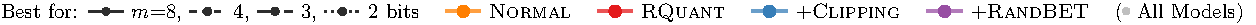
\includegraphics[width=1\textwidth]{c10_legend}
	\end{subfigure}
	}
	\vspace*{-14px}
	\caption{\textbf{Bit Error Robustness on \CifarT, \CifarH and \MNIST.} Average \RTE plotted against bit error rate $p$, both in \%. We considered various models (in {\color{gray}$\bullet$ gray}), corresponding to different $\wmax$ and $p$ during training. We explicitly plot the best model for each bit error rate: for \Normal ({\color{colorbrewer5}orange}), \Quant ({\color{colorbrewer1}red}), \Clipping ({\color{colorbrewer2}blue}) and \Random ({\color{colorbrewer4}violet}). Note that these might correspond to different $\wmax$ and $p$ (also across datasets). Across all approaches, we plot the per-error-rate best model in black: for $m = 8,4,3,2$ bits, depending on dataset. For $8$ bit and low bit error rates, \Clipping is often sufficient. However, for $4$ bit or higher bit error rates, \Random is crucial to keep \RTE low.}
	\label{fig:summary}
	\vspace*{-0.2cm}
\end{figure*}

\textbf{\Random Improves Robustness:}
%\label{subsec:experiments-randbet}
%
\Random, with weight clipping, further improves robustness and additionally generalizes across chips and voltages. \tabref{tab:randbet-robustness} shows results for weight clipping and \Random with $\wmax = 0.1$ and $m = 8,4$ bits precision. \Random is particularly effective against large bit error rates, \eg, $p = 1.5\%$, reducing \RTE from $12.22\%$ to $8.65\%$ ($m = 8$ bits). The effect is pronounced for $4$ bits or even lower precision, where models are generally less robust. The optimal combination of weight clipping and \Random depends on the bit error rate. For example, in \tabref{tab:clipping-robustness}, lowering $\wmax$ to $0.05$ reduces \RTE below \Random[$0.1$] with $p{=}1\%$ for some bit error rates.
We emphasize that \Random generalizes to lower bit errors than trained on, in stark contrast to the fixed-pattern training \Pattern. In \appref{subsec:supp-experiments-architectures}, we also show that \Random works on other architectures such as ResNet-50. On other datasets, \eg,\MNIST, \Random allows to operate at $p = 12.5\%$ bit error rate with $0.9\%$ \RTE and only $m = 2$ bits. At this point, weight clipping alone yields $90\%$ \RTE.

\textbf{\Random Generalizes to Profiled Bit Errors:}
%\label{subsec:experiments-generalization}
% 
\Random also generalizes to profiled bit errors from real chips. \tabref{tab:randbet-generalization} shows results on the two profiled chips of \figref{fig:errors}. Profiling was done at various voltage levels, resulting in different bit error rates. To simulate various weights to memory mappings, we apply various offsets before linearly mapping weights to the profiled SRAM arrays. \tabref{tab:randbet-generalization} reports average \RTE, showing that \Random generalizes quite well to these profiled bit errors. Regarding chip 1, \Random performs very well, even for large $p\approx 2.75$, as the bit error distribution of chip 1 largely matches our error model in \secref{sec:errors}, \cf \figref{fig:errors} (left). In contrast, with chip 2 we picked a more difficult bit error distribution which is strongly aligned along columns, potentially hitting many MSBs simultaneously. Thus, \RTE increases for chip 2 even for a lower bit error rate $p \approx 1.08$ (marked in {\color{colorbrewer1}red})
but energy savings are still possible without degrading prediction performance. 

\subsection{Summary and Discussion}
\label{subsec:experiments-discussion}
 
Our experiments are summarized in \figref{fig:summary}. We consider \Normal quantization vs. our robust quantization \Quant, various \Clipping and \Random models with different $\wmax$ and $p$ during training (indicated in {\color{gray}$\bullet$ gray}) and plot \RTE against bit error rate $p$ at test time. On all datasets \Quant outperforms \Normal. On \CifarT (left), \RTE increases significantly for \Quant ({\color{colorbrewer1}red}) starting at $p \approx 0.25\%$ bit error rate. While \Clipping ({\color{colorbrewer2}blue}) generally reduces \RTE, only \Random ({\color{colorbrewer4}violet}) can keep \RTE around $6\%$ or lower for a bit error rate of $p \approx 0.5\%$. The best model for each bit error rate $p$ (black and solid for $m = 8$) might vary. \CifarH is generally more difficult, while significantly higher bit error rates are possible on \MNIST. On \CifarT, \RTE increases slightly for $m = 4$. However, for $m = 3,2$ \RTE increases more significantly as clean \TE increases by $1-2\%$. % which likely due to our simple quantization. 
Nevertheless, \RTE only increases slightly for larger bit error rates $p$. It remains future work whether \Random with a more sophisticated (but robust) quantization scheme can enable low-voltage operation even for $m = 2$ bits. In all cases, \RTE increases monotonically, ensuring safe operation at higher voltages. The best trade-off between robustness and accuracy depends on the application: higher energy savings require a larger ``sacrifice'' in terms of \RTE.
Finally, \appref{subsec:supp-bound} provides a
confidence-interval based guarantee on how strongly \RTE is expected to deviate from the empirical results in \figref{fig:summary}.

Overall, the results in \figref{fig:summary} enable robust low-voltage operation \emph{without} requiring expensive error correcting codes (ECCs) or other circuit techniques \cite{ReagenISCA2016,ChandramoorthyHPCA2019}. Furthermore, our analysis applies both to DRAM, commonly off-chip, and SRAM, usually used as scratchpads on-chip of DNN accelerators. Compared to co-design \cite{KimDATE2018,KoppulaMICRO2019}, we do not require expensive expert knowledge or profiling infrastructure. Moreover, \Random improves over these approaches by generalizing across chips and voltages.
Besides \Random, we show that robust fixed-point quantization \emph{only with} weight clipping can provide reasonable robustness, \eg, for $p = 0.1\%$ on \CifarT. This is without sophisticated quantization scheme, \eg, with special treatment for outliers \cite{ZhuangCVPR2018,SungARXIV2015,ParkISCA2018}, and complementary to  \cite{MurthyARXIV2019,MerollaARXIV2016,SungARXIV2015,AlizadehICLR2020}, focusing merely on robustness \emph{to} quantization.
